\documentclass[12pt, letterpaper, twoside]{book}
\raggedbottom
\usepackage{graphicx}
\graphicspath{ {images/} }
\usepackage[utf8]{inputenc}
\usepackage{fullpage}
\usepackage[paperheight=11in,paperwidth=8.5in,margin=0in]{geometry}
\usepackage{amsmath}
\usepackage{listings}
\date{22nd May 2021}
\begin{document}
\begin{titlepage}
	\begin{center}
       \vspace*{5cm}
       \bfseries\Large
    	Assignment 1\\
    	Of\\
    	Modelling \& Simulation Lab (CS1052)\\
        \vskip1cm
        Masters of Technology in Computer Science And Engineering\\
        \vskip1cm
        submitted by\\
    	Arghya Bandyopadhyay\\
    	RollNo. 20CS4103\\
    	\vskip1cm
    	submitted to\\
    	Dr Nanda Dulal Jana\\
    	Assistant Professor\\
    	Dept. of CSE\\
    	\vskip1cm
    	
\includegraphics[width=4cm]{NITDGP}\\
    	National Institute of Technology, Durgapur\\
    \end{center}
\end{titlepage}

\begin{flushleft}
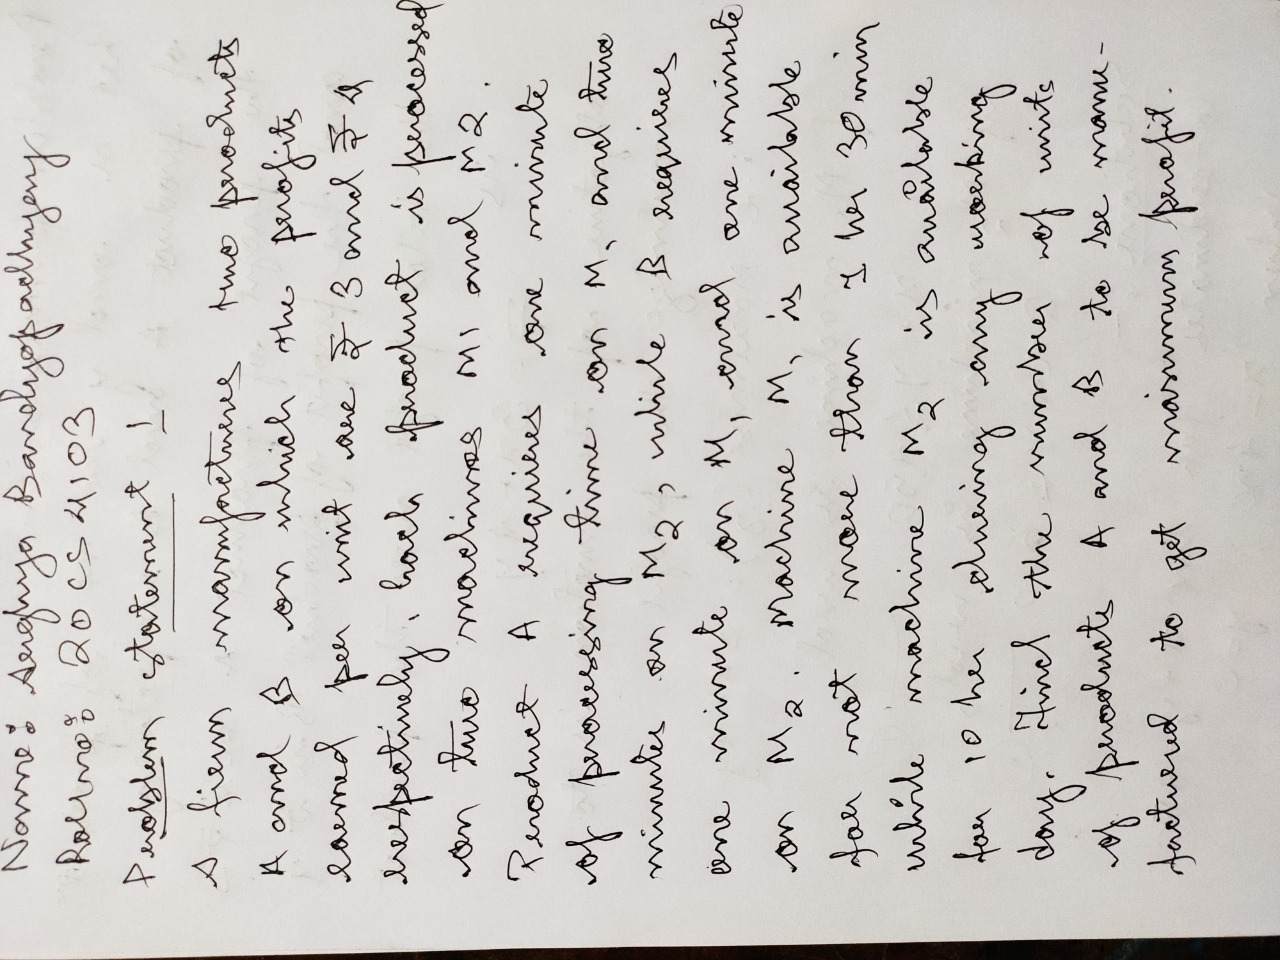
\includegraphics[width=\paperheight, height=8.49in, angle=270]{Page1}
\end{flushleft}
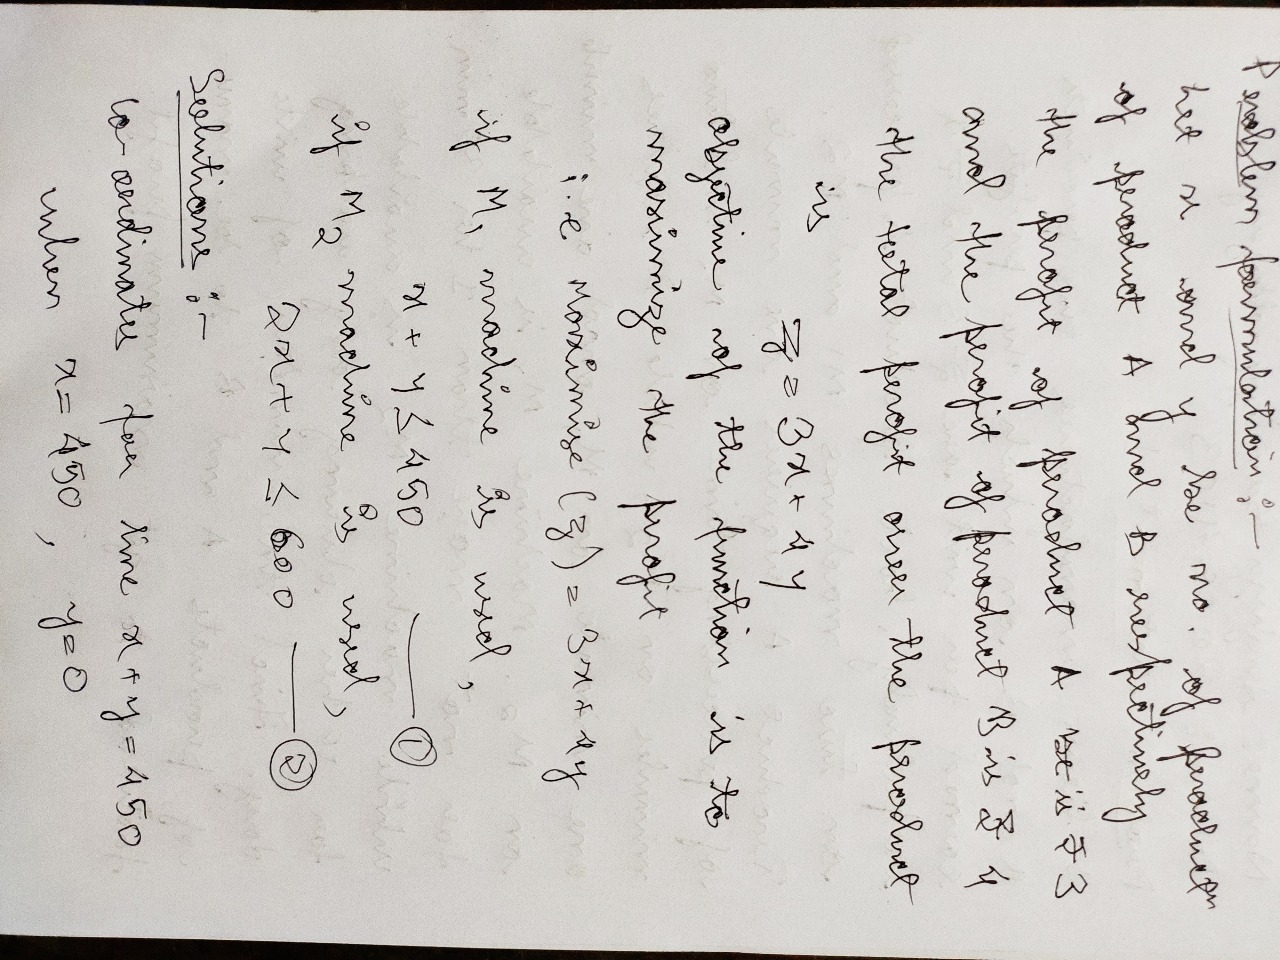
\includegraphics[width=\paperheight, height=\paperwidth, angle=90]{Page2}
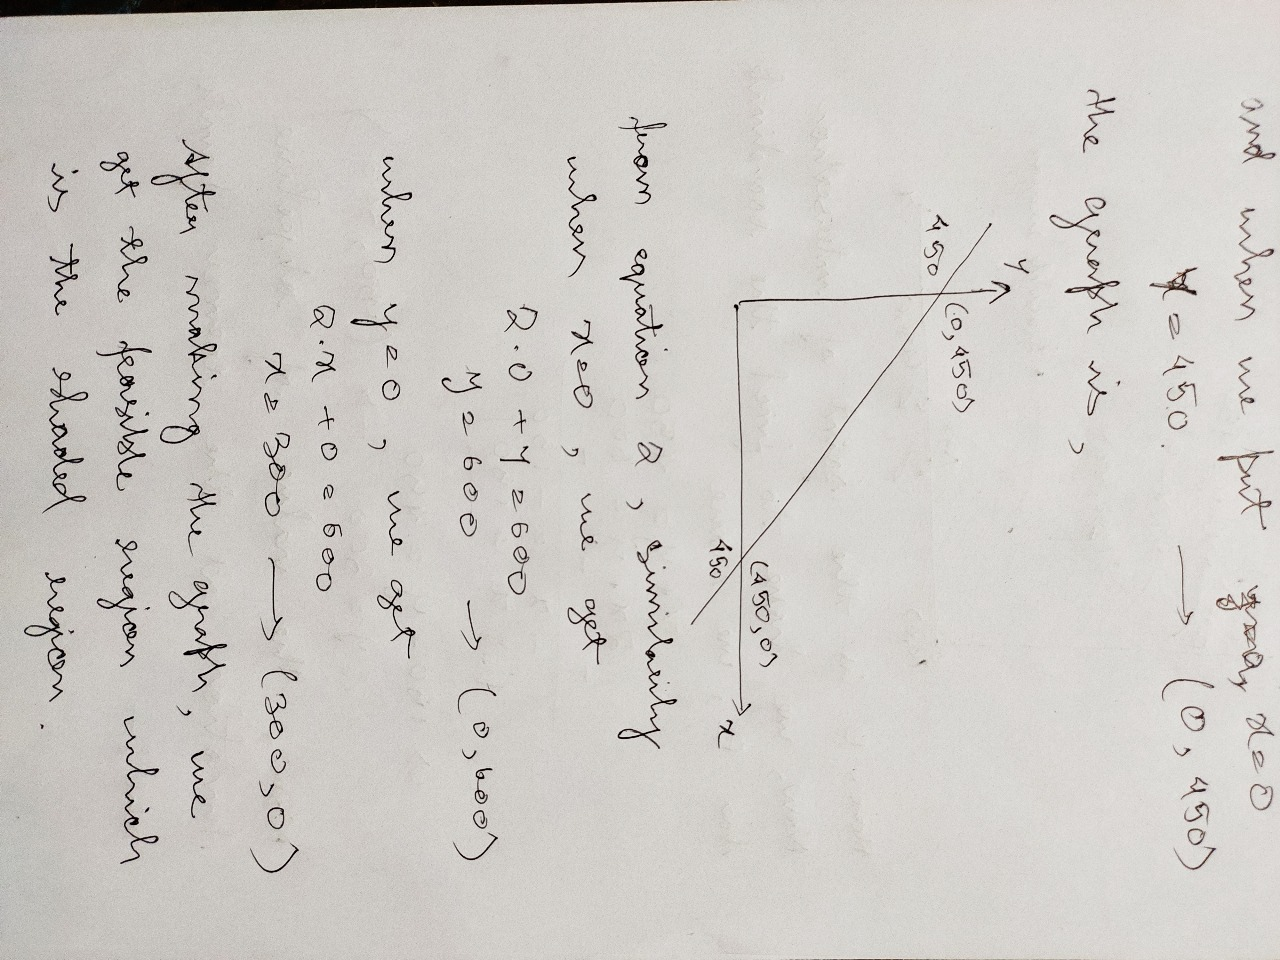
\includegraphics[width=\paperheight, height=\paperwidth, angle=90]{Page3}
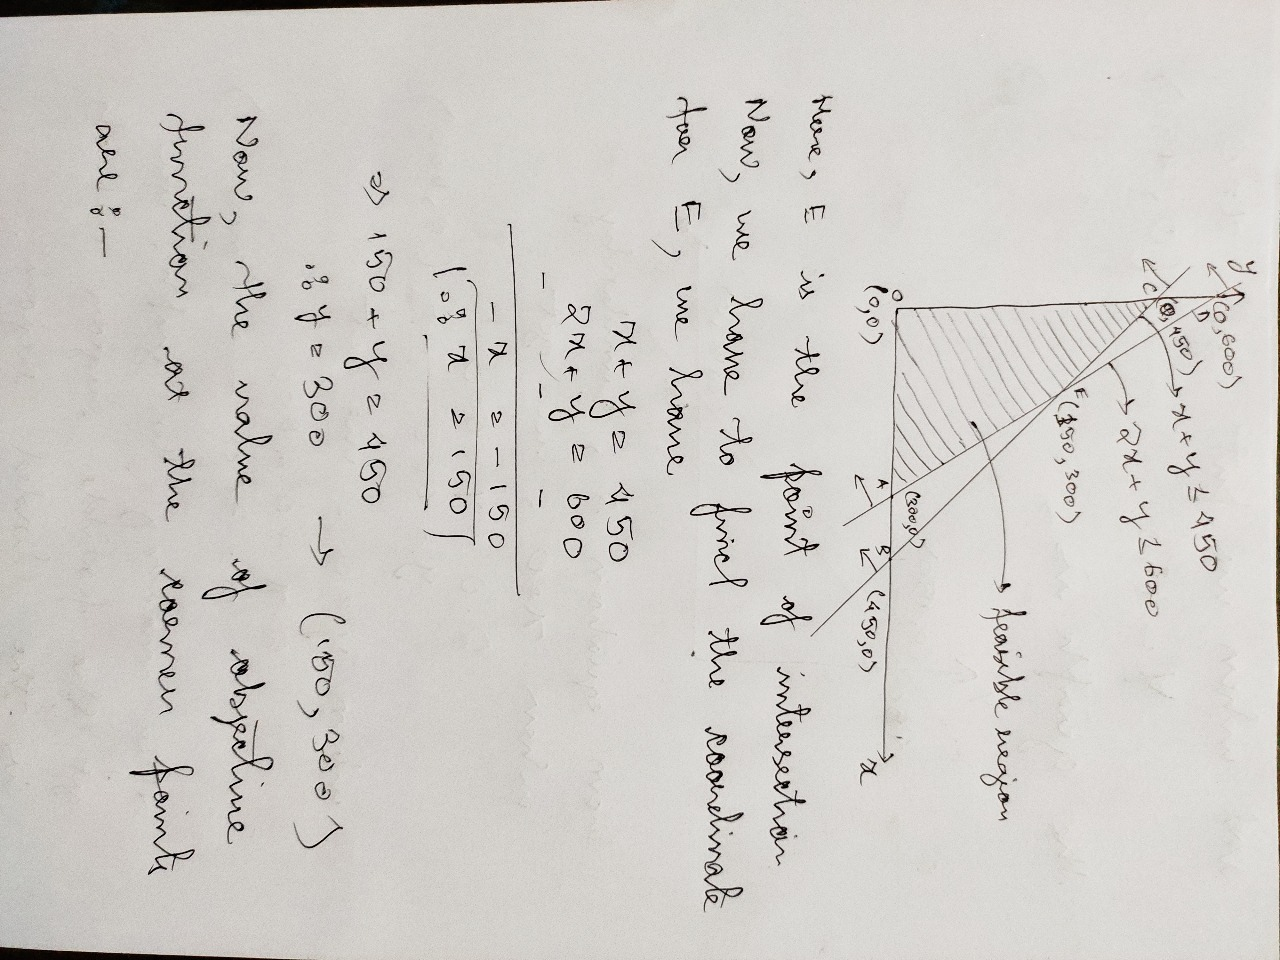
\includegraphics[width=\paperheight, height=\paperwidth, angle=90]{Page4}
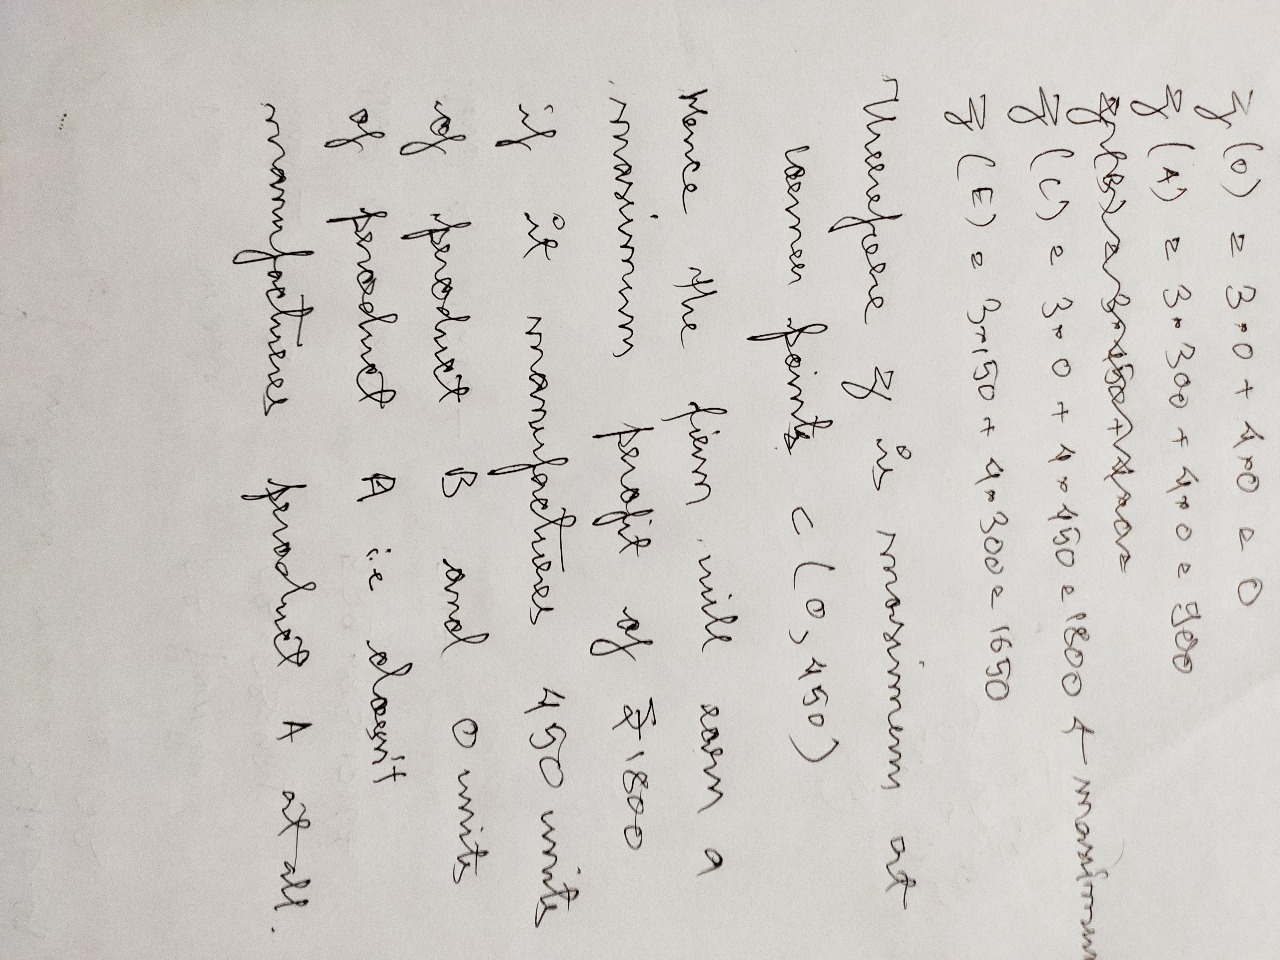
\includegraphics[width=\paperheight, height=\paperwidth, angle=90]{Page5}

\begin{lstlisting}

	Python Code:
	
	from shapely.geometry import LineString
	from matplotlib import pyplot as plt

	# main function
	if __name__ == '__main__':
	
		# The end point coordinates of the line for the equation 1
		x1 = [450, 0]
		y1 = [0, 450]
		
		# Plots the line for the equation 1
		plt.plot(x1, y1)
		
		# The end point coordinates of the line for the equation 2
		x2 = [300, 0]
		y2 = [0, 600]
		
		# Plots the line for the equation 2
		plt.plot(x2, y2)
		
		# Labels the axis and the plot
		plt.xlabel('No of production of A')
		plt.ylabel('No of production of B')
		plt.title('Plot for the problem 1')
		
		# Create the lines using the coordinates
		line1 = LineString([(450, 0), (0, 450)])
		line2 = LineString([(300, 0), (0, 600)])
		
		# Calculates the intersection and assigns it to the variable
		intersection = line1.intersection(line2)
		
		# Places a green colored circular disc on the coordinate specified
		plt.plot(*intersection.xy, 'go')
		
		# Places a blue colored star on the coordinate specified
		plt.plot(0, 450, 'b*')
		
		# Places a red colored star on the coordinate specified
		plt.plot(300, 0, 'r*')
		
		# Calculates the feasible regions dimensions
		p1, q1 = intersection.xy
		x = []
		y = []
		x.append(0)
		x.append(round(p1[0]))
		x.append(300)
		y.append(450)
		y.append(round(q1[0]))
		y.append(0)
		
		# Shades the feasible region
		plt.fill_between(x, y, color='blue', alpha=0.2)
		plt.text(260, 200, "x + y = 450")
		plt.text(55, 500, "2x + y = 600")
		
		# Opens the dialog showing the plot
		plt.show()
		print("Point of Intersection 1: ")
		print(p1[0])
		print(q1[0])
		z = []
		for i in range(len(x)):
			eqn = 3 * x[i] + 4 * y[i]
			z.append(eqn)
			print("Z = ", z)
		max_val = max(z)
		xy_index = z.index(max_val)
		print("The Value of Z ", max_val, 
			" at point (", x[xy_index], 
			",", y[xy_index], ")")
\end{lstlisting}
\begin{lstlisting}

	Output:
	
\end{lstlisting}
\begin{center}
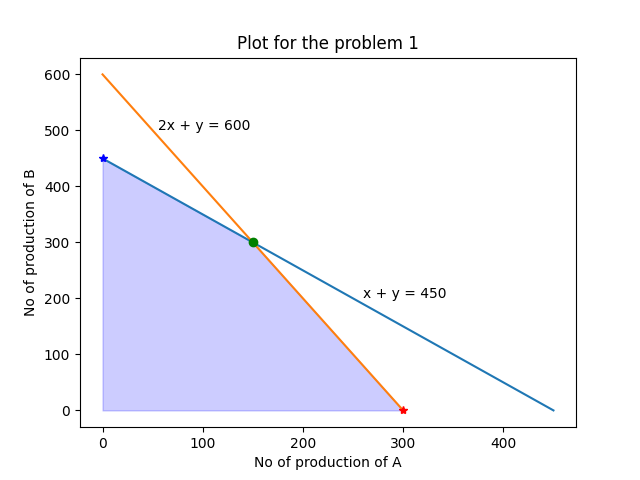
\includegraphics[height=400pt]{Plot1}
\end{center}
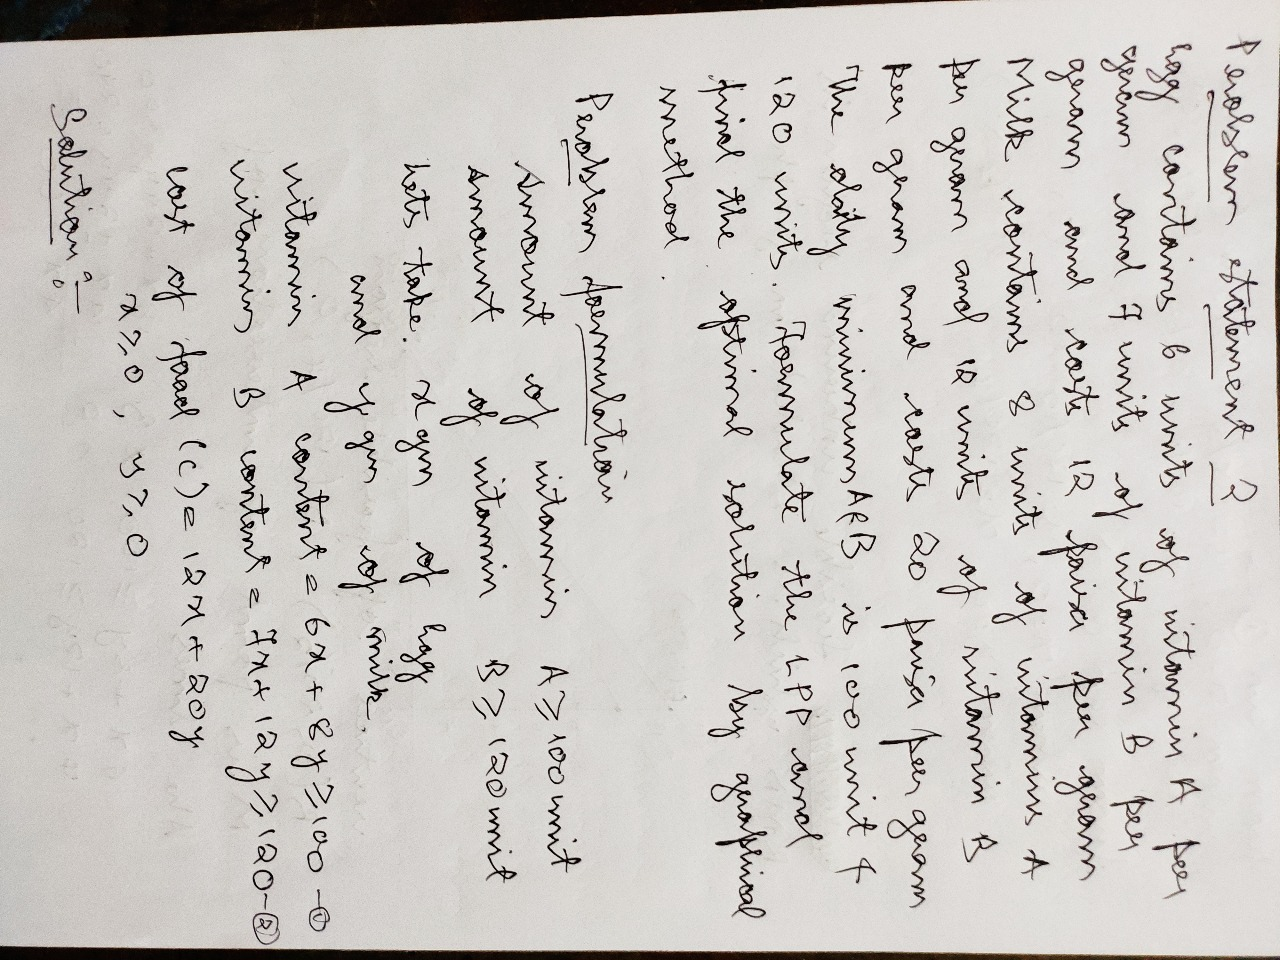
\includegraphics[width=\paperheight, height=\paperwidth, angle=90]{Page6}
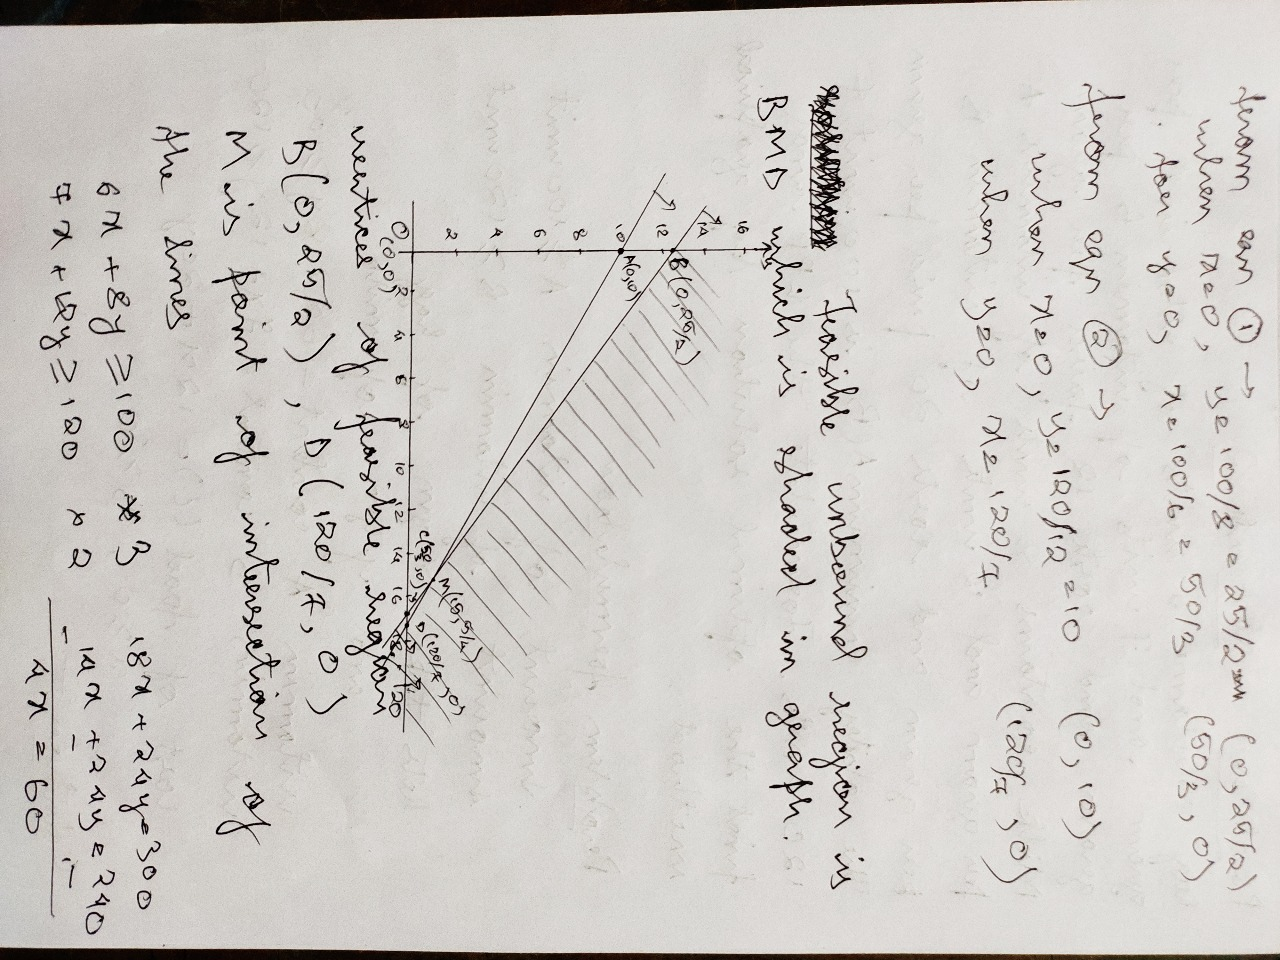
\includegraphics[width=\paperheight, height=\paperwidth, angle=90]{Page7}
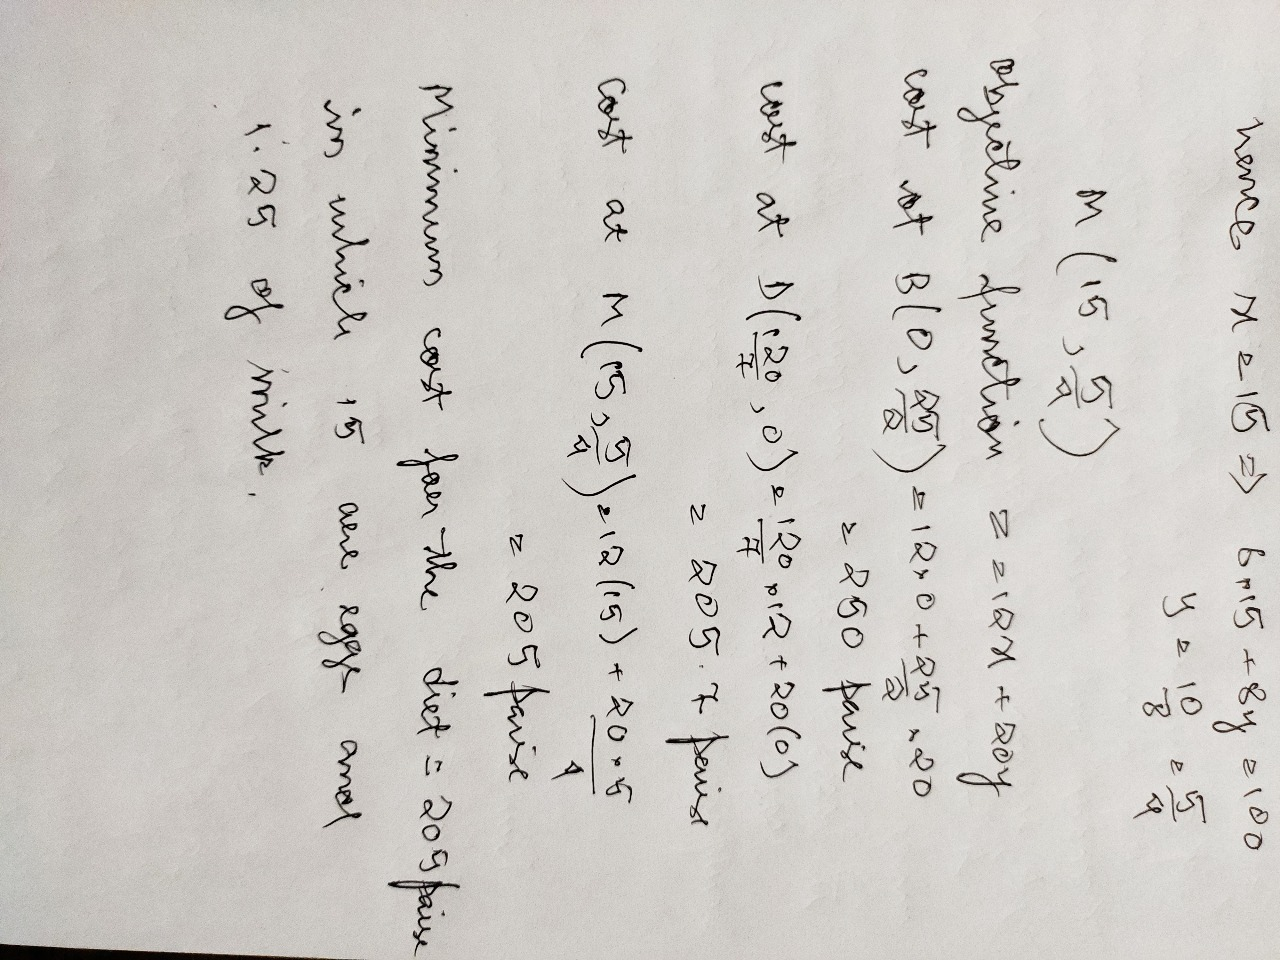
\includegraphics[width=\paperheight, height=\paperwidth, angle=90]{Page8}
\begin{lstlisting}

	Python Code:
	
	from shapely.geometry import LineString
	from matplotlib import pyplot as plt
	
	# main function
	if __name__ == '__main__':
		
		# The end point coordinates of the line for the equation 1
		x1 = [0,16.66]
		y1 = [12.5,0]
		
		# Plots the line for the equation 1
		plt.plot(x1, y1)
		
		# The end point coordinates of the line for the equation 2
		x2 = [17.14,0]
		y2 = [0,10]
		
		# Plots the line for the equation 2
		plt.plot(x2, y2)
		
		# Labels the axis and the plot
		plt.xlabel('Amount of Eggs in gms')
		plt.ylabel('Amount of Milk in gms')
		plt.title('Plot for the problem 2')
		
		# Create the lines using the coordinates
		line1 = LineString([(16.66,0),(0,12.5)])
		line2 = LineString([(17.14,0),(0,10)])
		
		# Calculates the intersection and assigns it to the variable
		# Places a green colored circular disc on the coordinate specified
		plt.plot(*intersection.xy, 'go')
		
		# Places a blue colored star on the coordinate specified
		plt.plot(0,12.5,'b*')
		plt.plot(17.14,0,'r*')
		
		# Calculates the feasible regions dimensions
		p1, q1 = intersection.xy
		x = []
		y = []
		x.append(0)
		x.append(round(p1[0],2))
		x.append(17.14)
		y.append(12.5)
		y.append(round(q1[0],2))
		y.append(0)
		
		# Shades the feasible region
		plt.fill_between(x,y,max(y),color='blue',alpha=0.2)
		plt.text(7,8,"6x + 8y = 100")
		
		plt.text(3,5,"7x + 12y = 120")
		
		# Opens the dialog showing the plot
		plt.show()
		print("Point of Intersection 1: ")
		print(round(p1[0],2))
		print(round(q1[0],2))
		z=[]
		for i in range(len(x)):
			eqn = 12*x[i] + 20*y[i]
			z.append(round(eqn,2))
			print("Z = ",z)
		min_val = min(z)
		xy_index = z.index(min_val)
		print("The Value of Z ",min_val,
			" at point (",x[xy_index],
			",",y[xy_index],")")
	    
\end{lstlisting}
\begin{lstlisting}

	Output:
	
\end{lstlisting}
\begin{center}
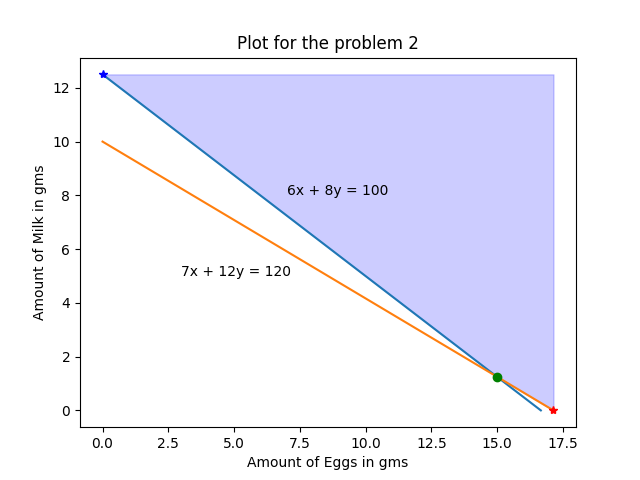
\includegraphics[height=400pt]{Plot2}
\end{center}
\end{document}
